The goal of JL is to presere $\ell_{2}$ distances. However, depending
on what property you care about, there will be different linear
dimensionality reduction techniques appropriate for your task. \\ 

\noindent Common linear dimensionality reduction techniques:
\begin{itemize}
\item RP (Random Projection)
\item PCA (Principal Component Analysis)
\item LDA (Linear Discriminate Analysis)
\item MDS (Multi-dimensional Scaling)
\item ICA/BSS (Independent Component Analysis/Blind Source Separation)
\item CCA (Canonical Correlation Analysis)
\item DML (Distance Metric Learning)
\item Factor (Factor Analysis)
\item NMF/MF ((Non-negative) Matrix Factorization)
\item Feature Selection
\end{itemize}

\section{RP (Random Projection)}
\subsubsection*{Method}
For random projection, $P\in \mathbb{R}^{d\times D}$ with $P_{ij} =
\mathcal{N}(0,1)$. i.e. 
\[
P = 
\begin{bmatrix}
    \mathcal{N}(0,1) & \mathcal{N}(0,1) & \dotsm\ \\
    \vdots & \ddots & \\
\end{bmatrix}
\]
If a projection matrix is wanted, apply Gram-Schmidt to $P$.

\subsection{Practical application}
PCA has time complexity $O(n^3)$, if we assume both the number of data
points and the number of features are equal to $n$. In practice, if we
are working with large amounts of data our first instinct to speed up
PCA might be to subsample the data, i.e. if our dataset has 10k
samples in $\mathbb{R}^{10k}$, randomly subsample 1k points and
perform PCA on this reduced dataset. However, the quality of the
$k^{\rm th}$ eigenvector of the subsampled data decays with respect to
the $k^{\rm th}$ eigenvector of the full dataset. While the first
eigenvector of the subsampled and full dataset will be similar, all
subsequent eigenvectors of the subsampled data will be of worsening
quality.  

The better approach to speeding up PCA is to first do a random
projection, and then perform PCA. While the distances between points
will be distorted within 1 $\pm$ $\epsilon$, the quality of the
eigenvectors will be better.

Random Projection plays a major role in processing images from
single-pixel cameras. These cameras use a method called compressive
sampling, which looks to reconstruct the optical signal. 
Specifically, random projection helps with a technique called 
smashed filters (as opposed to matched filters), which benefits from
the fact that random sampling preserves the original structure of the
data with high probability since it maintains inter-point distances. 
To learn more about this process, see "Single-Pixel Imaging via 
Compressive Sampling" \cite{duarte}.

\section{PCA~(Principal Component Analysis)}
\subsection{Outline}
Data: $x_1,x_2,...,x_n \in \mathbb{R}^d$\\

\noindent Goal: Find the best linear transformation $\phi:
\mathbb{R}^d \rightarrow \mathbb{R}^k$ that best maintains
reconstruction accuracy. Equivalently, minimize aggregate residual
error.\\ 

\noindent Define: $\Pi^k: \mathbb{R}^d \rightarrow \mathbb{R}^d$
minimize $\frac{1}{n} \sum_{i=1}^n ||x_i - \Pi^k (x_i)||^2$\\

\begin{figure}[h!]
\begin{center}
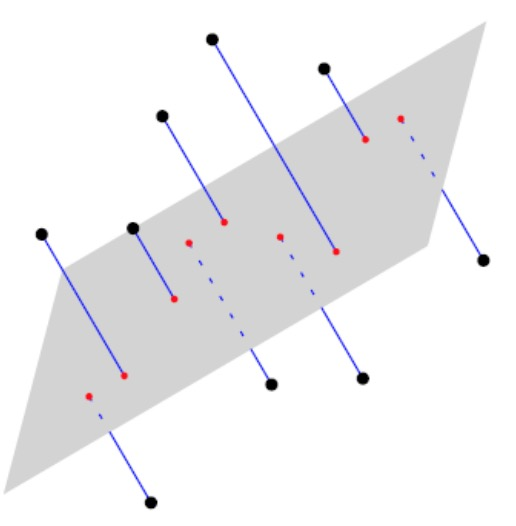
\includegraphics[width=0.5\textwidth]{chapter_6/files/projections.jpg}
\caption{An illustration of PCA}
\end{center}
\end{figure}
\subsubsection{Method}

A $k$ dimensional subspace can be represented by $q_1,...,q_k \in
\mathbb{R}^d$ orthonormal vectors.\\ 
The projection of any $x\in \mathbb{R}^d$ in the $span(q_1,...,q_k)$
is given by 
\[
\underbrace{(\sum_{i=1}^k q_i q_i^T)x}_{\Pi^k} = \sum_{i=1}^k
(q_i\cdot x)q_i 
\]
To represent it in $\mathbb{R}^k$ (using basis $q_1,...,q_k$) the
coefficients simply are: $(q_1,x),...,(q_k,x)$.\\ 
\subsection{The $k$ = 1 case}
In $k=1$ case, the objective is the following:\\

$\textrm{minimize}_{||q||=1} \frac{1}{n} \sum_{i=1}^n
||x_i - (qq^T)x_i||^2$\\

\noindent Equivalently,\\

$\textrm{maximize}_{||q||=1}q^T(\frac{1}{n} XX^T)q$, \\

\noindent where $\frac{1}{n}XX^T$ is the covariance of data, if the
data is mean-centered. The solution is the top eigenvector
$(1/n)XX^T$.\\ 

\noindent \textbf{Remark}: For any $q$, the quadratic form
$q^T(\frac{1}{n}XX^T)q$ is the empirical variance of data in the
direction $q$. 
\subsubsection{General $k$ case}
The general $k$ case is similar and the solution is basically the top
$k$ eigenvectors of the matrix $XX^T$.\\ 

\section{LDA~(Linear Discriminate Analysis)}
\subsection{Motivation}
The goal of PCA is to minimize the reconstruction error. However, this
is not necessarily going to help for classification purposes. 
\subsection{Method}
Define $\mu_1=\frac{1}{|C_1|} \sum_{x\in C_1} x$ and
$\mu_2=\frac{1}{|C_2|} \sum_{x\in C_2} x$. Define $\bar{\mu}_1=w^T
\mu_1$ and $\bar{\mu}_2=w^T \mu_2$\\ 
One intuitive formulation would be:
\[
\max_{w,s.t.||w||=1} L(w) = |\bar{\mu}_1 - \bar{\mu}_2| = |w^T\mu_1 - w^T\mu_2|
\]
It is easy to see that $w^*=\frac{\mu_1 - \mu_2}{||\mu_1-\mu_2||}$.\\

\noindent Problem: Maintaining the distance between the means is not
sufficient. What we want are for the: 
\begin{itemize}
\item class means to be as far as possible after projection, and
\item class variances to be as small as possible.
\end{itemize}
After projection, denote $\bar{s}_1^2 = \sum_{\bar{x}\in C_1}
(\bar{x}-\bar{\mu}_1)^2$, $\bar{s}_2^2 = \sum_{\bar{x}\in C_2}
(\bar{x}-\bar{\mu}_2)^2$. The formulation according to our criteria
would be the following: 
\[
\max_{w} L(w)=\frac{(\bar{\mu}_1 - \bar{\mu}_2)^2}{\bar{s}_1^2+\bar{s}_2^2}
\]
We will expand each term in this equation in the following:\\
\begin{align*}
\bar{s}_1^2
&= \sum_{\bar{x}\in C_1} (\bar{x}-\bar{\mu}_1)^2\\
&= \sum_{\bar{x}\in C_1} (w^Tx-w^T\mu_1)^2\\
&= w^T\Big (\sum_{\bar{x}\in C_1} (x-\mu_1)(x-\mu_1)^T \Big ) w\\
&= w^TS_1w \textrm{ where } S_1 \textrm{ is the scatter matrix for }1
\end{align*}
Similarly, $\bar{s}_2^2=w^TS_2w$\\
\begin{align*}
(\bar{\mu}_1-\bar{\mu}_2)^2
&= (w^T (\mu_1 - \mu_2))^2\\
&= w^T(\mu_1-\mu_2)(\mu_1-\mu_2)^Tw\\
&= w^TS_Bw \textrm{ where } S_B \textrm{ is the between class scatter
    matrix} 
\end{align*}
Note: rank of $S_B = 1$.\\
Thus,
\[
L(w)=\frac{w^T S_B w}{w^T S_w w}
\]
It follows that it has derivative (if we ignore its denominator):
\[
\frac{d}{dw}L(w)=w^TS_w w2S_B w - w^T S_B w 2 S_w w
\]
When we divide it by $2w^TS_ww$, we get:
\[
S_Bw - \frac{w^T S_B w}{w^T S_w w} (S_w w)=S_Bw - L(w)(S_w w)
\]
If we let it equal to 0, we get:
\[
S_B w = S_w L(w) w \Leftrightarrow S_w^{-1} S_B w = L(w) w
\]
Maximizing $L(w) \Leftrightarrow$ finding eigenvector corresponding to
the largest eigenvalues of $S_w^{-1} S_B$.\\ 

\noindent \textbf{Remark}: When you have $c$-classes, LDA will find a
$c-1$ subspace. \\ 

\section{MDS~(Multi-dimensional Scaling)}
MDS is useful when you don't have a Euclidean representation of the
data, and wish to come up with one based on distances between data
points. There are three types of MDS: 
\begin{itemize}
\item classical MDS
\item metric MDS
\item non-metric MDS
\end{itemize}
Here, we are mostly going to discuss metric MDS.\\
\subsection{Metric MDS method}
Given a distance matrix $P \in \mathbb{R}^{n\times n}$, define the
``stress function", for $x_i \in \mathbb{R}^k \ \forall i=1,...,n$, to
be the following: 
\[
S(x_1,...,x_n) = \sum_{i<j}(||x_i-x_j||-p_{ij})^2
\]
We want to minimize the stress function over the data points $x_1,...,x_n$.\\
The problem can be formulated as the following:\\
\begin{align*}
&\min S(x_1,...,x_n)\\
&s.t. \sum x_i = 0
\end{align*}
There is no easy way to write this as an eigenvalue problem, so to
solve this we can simply do any gradient based optimization.\\ 

\subsection{Non-metric MDS}
The goal on non-metric MDS is to maintain the order of distances
between data points. For example, if $x_{i}$ is closer to $x_{j}$ than
$x_{k}$, then maintain this ordering. Can make $||x_{i} - x_{j}||$
into any monotonic function. 
